% Options for packages loaded elsewhere
\PassOptionsToPackage{unicode}{hyperref}
\PassOptionsToPackage{hyphens}{url}
\PassOptionsToPackage{dvipsnames,svgnames,x11names}{xcolor}
%
\documentclass[
  letterpaper,
  DIV=11,
  numbers=noendperiod]{scrreprt}

\usepackage{amsmath,amssymb}
\usepackage{iftex}
\ifPDFTeX
  \usepackage[T1]{fontenc}
  \usepackage[utf8]{inputenc}
  \usepackage{textcomp} % provide euro and other symbols
\else % if luatex or xetex
  \usepackage{unicode-math}
  \defaultfontfeatures{Scale=MatchLowercase}
  \defaultfontfeatures[\rmfamily]{Ligatures=TeX,Scale=1}
\fi
\usepackage{lmodern}
\ifPDFTeX\else  
    % xetex/luatex font selection
\fi
% Use upquote if available, for straight quotes in verbatim environments
\IfFileExists{upquote.sty}{\usepackage{upquote}}{}
\IfFileExists{microtype.sty}{% use microtype if available
  \usepackage[]{microtype}
  \UseMicrotypeSet[protrusion]{basicmath} % disable protrusion for tt fonts
}{}
\makeatletter
\@ifundefined{KOMAClassName}{% if non-KOMA class
  \IfFileExists{parskip.sty}{%
    \usepackage{parskip}
  }{% else
    \setlength{\parindent}{0pt}
    \setlength{\parskip}{6pt plus 2pt minus 1pt}}
}{% if KOMA class
  \KOMAoptions{parskip=half}}
\makeatother
\usepackage{xcolor}
\setlength{\emergencystretch}{3em} % prevent overfull lines
\setcounter{secnumdepth}{5}
% Make \paragraph and \subparagraph free-standing
\ifx\paragraph\undefined\else
  \let\oldparagraph\paragraph
  \renewcommand{\paragraph}[1]{\oldparagraph{#1}\mbox{}}
\fi
\ifx\subparagraph\undefined\else
  \let\oldsubparagraph\subparagraph
  \renewcommand{\subparagraph}[1]{\oldsubparagraph{#1}\mbox{}}
\fi


\providecommand{\tightlist}{%
  \setlength{\itemsep}{0pt}\setlength{\parskip}{0pt}}\usepackage{longtable,booktabs,array}
\usepackage{calc} % for calculating minipage widths
% Correct order of tables after \paragraph or \subparagraph
\usepackage{etoolbox}
\makeatletter
\patchcmd\longtable{\par}{\if@noskipsec\mbox{}\fi\par}{}{}
\makeatother
% Allow footnotes in longtable head/foot
\IfFileExists{footnotehyper.sty}{\usepackage{footnotehyper}}{\usepackage{footnote}}
\makesavenoteenv{longtable}
\usepackage{graphicx}
\makeatletter
\def\maxwidth{\ifdim\Gin@nat@width>\linewidth\linewidth\else\Gin@nat@width\fi}
\def\maxheight{\ifdim\Gin@nat@height>\textheight\textheight\else\Gin@nat@height\fi}
\makeatother
% Scale images if necessary, so that they will not overflow the page
% margins by default, and it is still possible to overwrite the defaults
% using explicit options in \includegraphics[width, height, ...]{}
\setkeys{Gin}{width=\maxwidth,height=\maxheight,keepaspectratio}
% Set default figure placement to htbp
\makeatletter
\def\fps@figure{htbp}
\makeatother
% definitions for citeproc citations
\NewDocumentCommand\citeproctext{}{}
\NewDocumentCommand\citeproc{mm}{%
  \begingroup\def\citeproctext{#2}\cite{#1}\endgroup}
\makeatletter
 % allow citations to break across lines
 \let\@cite@ofmt\@firstofone
 % avoid brackets around text for \cite:
 \def\@biblabel#1{}
 \def\@cite#1#2{{#1\if@tempswa , #2\fi}}
\makeatother
\newlength{\cslhangindent}
\setlength{\cslhangindent}{1.5em}
\newlength{\csllabelwidth}
\setlength{\csllabelwidth}{3em}
\newenvironment{CSLReferences}[2] % #1 hanging-indent, #2 entry-spacing
 {\begin{list}{}{%
  \setlength{\itemindent}{0pt}
  \setlength{\leftmargin}{0pt}
  \setlength{\parsep}{0pt}
  % turn on hanging indent if param 1 is 1
  \ifodd #1
   \setlength{\leftmargin}{\cslhangindent}
   \setlength{\itemindent}{-1\cslhangindent}
  \fi
  % set entry spacing
  \setlength{\itemsep}{#2\baselineskip}}}
 {\end{list}}
\usepackage{calc}
\newcommand{\CSLBlock}[1]{\hfill\break\parbox[t]{\linewidth}{\strut\ignorespaces#1\strut}}
\newcommand{\CSLLeftMargin}[1]{\parbox[t]{\csllabelwidth}{\strut#1\strut}}
\newcommand{\CSLRightInline}[1]{\parbox[t]{\linewidth - \csllabelwidth}{\strut#1\strut}}
\newcommand{\CSLIndent}[1]{\hspace{\cslhangindent}#1}

\KOMAoption{captions}{tableheading}
\makeatletter
\@ifpackageloaded{bookmark}{}{\usepackage{bookmark}}
\makeatother
\makeatletter
\@ifpackageloaded{caption}{}{\usepackage{caption}}
\AtBeginDocument{%
\ifdefined\contentsname
  \renewcommand*\contentsname{Table of contents}
\else
  \newcommand\contentsname{Table of contents}
\fi
\ifdefined\listfigurename
  \renewcommand*\listfigurename{List of Figures}
\else
  \newcommand\listfigurename{List of Figures}
\fi
\ifdefined\listtablename
  \renewcommand*\listtablename{List of Tables}
\else
  \newcommand\listtablename{List of Tables}
\fi
\ifdefined\figurename
  \renewcommand*\figurename{Figure}
\else
  \newcommand\figurename{Figure}
\fi
\ifdefined\tablename
  \renewcommand*\tablename{Table}
\else
  \newcommand\tablename{Table}
\fi
}
\@ifpackageloaded{float}{}{\usepackage{float}}
\floatstyle{ruled}
\@ifundefined{c@chapter}{\newfloat{codelisting}{h}{lop}}{\newfloat{codelisting}{h}{lop}[chapter]}
\floatname{codelisting}{Listing}
\newcommand*\listoflistings{\listof{codelisting}{List of Listings}}
\makeatother
\makeatletter
\makeatother
\makeatletter
\@ifpackageloaded{caption}{}{\usepackage{caption}}
\@ifpackageloaded{subcaption}{}{\usepackage{subcaption}}
\makeatother
\ifLuaTeX
  \usepackage{selnolig}  % disable illegal ligatures
\fi
\usepackage{bookmark}

\IfFileExists{xurl.sty}{\usepackage{xurl}}{} % add URL line breaks if available
\urlstyle{same} % disable monospaced font for URLs
\hypersetup{
  pdftitle={Cap 18 Validation},
  pdfauthor={Cole Miller},
  colorlinks=true,
  linkcolor={blue},
  filecolor={Maroon},
  citecolor={Blue},
  urlcolor={Blue},
  pdfcreator={LaTeX via pandoc}}

\title{Cap 18 Validation}
\author{Cole Miller}
\date{2024-10-18}

\begin{document}
\maketitle

\renewcommand*\contentsname{Table of contents}
{
\hypersetup{linkcolor=}
\setcounter{tocdepth}{2}
\tableofcontents
}
\bookmarksetup{startatroot}

\chapter{Preface}\label{preface}

\bookmarksetup{startatroot}

\chapter{Cap18 Validation Summary}\label{cap18-validation-summary}

Cap18 is a TxDOT specialized structural analysis program using a
discrete element model that produces envelopes of maximum bending and
shear forces acting on bridge bent caps. HDR uses this software heavily
in the bent design process, so validation of this tool is necessary.
Since there is no access to the underlying code, validation must be
approached differently compared to internal tools. This document will
attempt to provide an outline for the process of validating the Cap18
program.

\section{Cap18 Inputs}\label{cap18-inputs}

This next section will get into the details of what the Cap18 program
is. It will try to stay concise. However, there are many inputs to the
program, and it is important to list out all of them in order to
determine the amount of options available.

The Cap18 program allows the user to provide a number of different
inputs. These inputs are provided to the program through a ``*.dat''
file. This input file is simply a text file that the program can parse
and then execute. The file has a specific format that is separated by
different ``cards''. There are 4 different types of cards. - Comment
Cards - Header Cards - Problem Cards - Table Cards The specific order of
these cards allows the program to know the current card as it steps
through each line. Each card is a single line in the input file that
contains multiple inputs the program can read. The multiple inputs are
separated by the position on the line (ie the first input will be a
certain range of characters in the beginning of the line). An input does
not have to fill the entire range of characters for that specific input.
This range allowance for each input will not be checked directly.
Although with the different bents, there will be enough disparity among
the inputs to that some level of checking will be done indirectly. A
summary of the cards and their list of inputs will now be discussed in
more detail to determine the brevity of the check that is needed.

\subsection{Comment Cards}\label{comment-cards}

Comment cards begin with a dollar sign (\$) and these lines are for the
users own documentation purposes. These cards are ignored by the Cap18
program. No checking is needed here.

\subsection{Header Cards}\label{header-cards}

Header cards are sort of comment cards, but the Cap18 program needs them
to run. These cards only contain general project information that does
not affect the results. The same headers will be provided to each run.
No checking is needed here.

\subsection{Problem Cards}\label{problem-cards}

Problem cards contain 3 inputs. - Problem number - Unit Code -
Description From the problem card inputs, unit code is the only one that
will affect results. However only the US Customary unit code will be
checked.

\subsection{Table Cards}\label{table-cards}

\subsubsection{Table 1}\label{table-1}

Table 1 card contains 9 inputs. - Print stringer reaction report - Keep
Envelopes from prior problem - Keep prior Table 2 - Keep prior Table 3 -
Keep prior Table 4 - Number of cards for Table 4 - Keep envelopes from
random lane - Print options - Skew angle

\subsubsection{Table 2}\label{table-2}

Table 2 has two cards Table2a and Table 2b.

Table 2a has 9 inputs. - number of slab increments - increment length -
number of total moving increments - start station of moving load - end
station of moving load - step size of moving increments - analysis
option - dead load factor - live load factor

Table 2b has 7 inputs. - overlay factor - max lanes loaded - multiple
presence factor for 1 lane - multiple presence factor for 2 lanes -
multiple presence factor for 3 lanes - multiple presence factor for 4
lanes - multiple presence factor for 5 lanes

\subsubsection{Table 3}\label{table-3}

Table 3 has a varied number of inputs depending on the problem. However,
they can be classified into 11 different inputs - number of lanes -
number of stringers - number of supports - number of moment points -
station at left lane - stations at right lane - station at stringers -
station at supports - station at moment points - station at shear points

\subsubsection{Table 4}\label{table-4}

Table 4 has a varied number of inputs, and they can be classified into 8
different inputs. - station from - station to - cont'd - bending
stiffness of cap - slab and sidewalk loads - cap and stringer loads -
moving loads - overlay loads

To validate Cap18, the program will be run for a number of various
bents. These results will then be compared against one of HDRs validated
software programs, LARSA. The different bent configurations will be
discussed below. At the end, a summary of the different bent
configurations and their inputs into the cap18 program will be shown.
The goal is for each input into the Cap18 program to at least have 1
different value across all the different configurations.

\section{Multi-Column Bents - No
Skew}\label{multi-column-bents---no-skew}

Here are a list of the bent configurations that fall into the above
category. - 24' roadway and bent with 3 columns - 40' roadway and bent
with 3 columns - 44' roadway and bent with 4 columns (Tx62 girders)

\section{Multi-Column Bents - With
Skew}\label{multi-column-bents---with-skew}

Here are a list of the bent configurations that fall into the above
category. - 24' roadway and bent with 3 columns 15, 30, 45 - 24' roadway
and bent with 3 columns 15, 30, 45 - 44' roadway and bent with 4 columns
(Tx62 girders) 15, 30, 45

\section{Single Column Bents}\label{single-column-bents}

\bookmarksetup{startatroot}

\chapter{Four Column Bent Analysis
Comparison}\label{four-column-bent-analysis-comparison}

A typical 4-column bent was run and analyzed with both Cap18 and LARSA.
Results between the two were fairly close, with Cap18 having more
conservative values in the maximum and minimum areas.

\section{Cap18 Results}\label{cap18-results}

\subsection{Dead Load Results (SRV)}\label{dead-load-results-srv}

\begin{figure}[H]

{\centering \includegraphics{index_files/mediabag/02_four_col_bent_files/figure-pdf/cell-5-output-1.pdf}

}

\caption{Cap18: DL Shear and Moment Diagrams}

\end{figure}%

\subsection{Envelopes of Maximum Values
(SRV)}\label{envelopes-of-maximum-values-srv}

\begin{figure}[H]

{\centering \includegraphics{index_files/mediabag/02_four_col_bent_files/figure-pdf/cell-7-output-1.pdf}

}

\caption{Cap18: Service Shear and Moment Envelope Diagrams}

\end{figure}%

\subsection{Maximum Support Reactions
(SRV)}\label{maximum-support-reactions-srv}

\begin{table}
\caption{Cap18: Service Reactions}\tabularnewline

\centering
\begin{tabular}{r|cccc}
    & sta & dist & max\_reaction & min\_reaction\\
    \hline
    & Int64 & Float64 & Float64 & Float64\\
    \hline
    1 & 8 & 4.0 & 376.5 & 229.2 \\
    2 & 32 & 16.0 & 441.0 & 245.3 \\
    3 & 56 & 28.0 & 441.0 & 245.3 \\
    4 & 80 & 40.0 & 376.5 & 229.2 \\
\end{tabular}
\end{table}

\subsection{Envelopes of Maximum Values
(STR)}\label{envelopes-of-maximum-values-str}

\begin{figure}[H]

{\centering \includegraphics{index_files/mediabag/02_four_col_bent_files/figure-pdf/cell-10-output-1.pdf}

}

\caption{Cap18: Strength Shear and Moment Envelope Diagrams}

\end{figure}%

\subsection{Maximum Support Reactions
(STR)}\label{maximum-support-reactions-str}

\begin{table}
\caption{Cap18: Strength Reactions}\tabularnewline

\centering
\begin{tabular}{r|cccc}
    & sta & dist & max\_reaction & min\_reaction\\
    \hline
    & Int64 & Float64 & Float64 & Float64\\
    \hline
    1 & 8 & 4.0 & 540.9 & 283.0 \\
    2 & 32 & 16.0 & 643.3 & 300.9 \\
    3 & 56 & 28.0 & 643.3 & 300.9 \\
\end{tabular}
\end{table}

\section{LARSA Results}\label{larsa-results}

\subsection{Dead Load Results}\label{dead-load-results}

\begin{figure}[H]

{\centering \includegraphics{index_files/mediabag/02_four_col_bent_files/figure-pdf/cell-14-output-1.pdf}

}

\caption{LARSA: DL Shear and Moment Diagrams}

\end{figure}%

\subsection{Envelopes of Maximum Values
(SRV)}\label{envelopes-of-maximum-values-srv-1}

\begin{figure}[H]

{\centering \includegraphics{index_files/mediabag/02_four_col_bent_files/figure-pdf/cell-16-output-1.pdf}

}

\caption{LARSA: Service Shear and Moment Envelope Diagrams}

\end{figure}%

\subsection{Maximum Support Reactions
(SRV)}\label{maximum-support-reactions-srv-1}

\begin{table}
\caption{Service Reactions}\tabularnewline

\centering
\begin{tabular}{r|cccc}
    & sta & dist & max\_reaction & min\_reaction\\
    \hline
    & Int64 & Float64 & Float64 & Float64\\
    \hline
    1 & 8 & 4.0 & 376.619 & 229.487 \\
    2 & 32 & 16.0 & 439.42 & 247.414 \\
    3 & 56 & 28.0 & 439.42 & 247.414 \\
    4 & 80 & 40.0 & 376.577 & 229.49 \\
\end{tabular}
\end{table}

\subsection{Envelopes of Maximum Values
(STR)}\label{envelopes-of-maximum-values-str-1}

\begin{figure}[H]

{\centering \includegraphics{index_files/mediabag/02_four_col_bent_files/figure-pdf/cell-19-output-1.pdf}

}

\caption{LARSA: Strength Shear and Moment Envelope Diagrams}

\end{figure}%

\subsection{Maximum Support Reactions
(STR)}\label{maximum-support-reactions-str-1}

\begin{table}
\caption{LARSA: Strength Reactions}\tabularnewline

\centering
\begin{tabular}{r|cccc}
    & sta & dist & max\_reaction & min\_reaction\\
    \hline
    & Int64 & Float64 & Float64 & Float64\\
    \hline
    1 & 8 & 4.0 & 541.086 & 283.606 \\
    2 & 32 & 16.0 & 604.078 & 304.531 \\
    3 & 56 & 28.0 & 604.078 & 304.531 \\
    4 & 80 & 40.0 & 541.013 & 283.611 \\
\end{tabular}
\end{table}

\section{Comparison}\label{comparison}

\subsection{Dead Load Results (SRV)}\label{dead-load-results-srv-1}

\begin{figure}[H]

{\centering \includegraphics{index_files/mediabag/02_four_col_bent_files/figure-pdf/cell-22-output-1.pdf}

}

\caption{Comparison: DL Shear and Moment Diagrams}

\end{figure}%

\begin{figure}[H]

{\centering \includegraphics{index_files/mediabag/02_four_col_bent_files/figure-pdf/cell-23-output-1.pdf}

}

\caption{Comparison: DL Shear and Moment Difference}

\end{figure}%

\subsection{Envelopes of Maximum Values
(SRV)}\label{envelopes-of-maximum-values-srv-2}

\begin{figure}[H]

{\centering \includegraphics{index_files/mediabag/02_four_col_bent_files/figure-pdf/cell-24-output-1.pdf}

}

\caption{Comparison: Service Shear and Moment Envelope Diagrams}

\end{figure}%

\begin{figure}[H]

{\centering \includegraphics{index_files/mediabag/02_four_col_bent_files/figure-pdf/cell-25-output-1.pdf}

}

\caption{Comparison: Service Shear and Moment Envelope Difference}

\end{figure}%

\subsection{Maximum Support Reactions
(SRV)}\label{maximum-support-reactions-srv-2}

\begin{figure}[H]

{\centering \includegraphics{index_files/mediabag/02_four_col_bent_files/figure-pdf/cell-26-output-1.pdf}

}

\caption{Comparison: Service Reactions}

\end{figure}%

\subsection{Envelopes of Maximum Values
(STR)}\label{envelopes-of-maximum-values-str-2}

\begin{figure}[H]

{\centering \includegraphics{index_files/mediabag/02_four_col_bent_files/figure-pdf/cell-27-output-1.pdf}

}

\caption{Comparison: Strength Shear and Moment Envelope Diagrams}

\end{figure}%

\begin{figure}[H]

{\centering \includegraphics{index_files/mediabag/02_four_col_bent_files/figure-pdf/cell-28-output-1.pdf}

}

\caption{Comparison: Strength Shear and Moment Envelope Difference}

\end{figure}%

\bookmarksetup{startatroot}

\chapter{Four Column Bent Analysis
Comparison}\label{four-column-bent-analysis-comparison-1}

A typical 4-column bent was run and analyzed with both Cap18 and LARSA.
Results between the two were fairly close, with Cap18 having more
conservative values in the maximum and minimum areas.

\section{Cap18 Results}\label{cap18-results-1}

\subsection{Dead Load Results (SRV)}\label{dead-load-results-srv-2}

\begin{figure}[H]

{\centering \includegraphics{index_files/mediabag/03_six_col_bent_files/figure-pdf/cell-5-output-1.pdf}

}

\caption{Cap18: DL Shear and Moment Diagrams}

\end{figure}%

\subsection{Envelopes of Maximum Values
(SRV)}\label{envelopes-of-maximum-values-srv-3}

\begin{figure}[H]

{\centering \includegraphics{index_files/mediabag/03_six_col_bent_files/figure-pdf/cell-7-output-1.pdf}

}

\caption{Cap18: Service Shear and Moment Envelope Diagrams}

\end{figure}%

\subsection{Maximum Support Reactions
(SRV)}\label{maximum-support-reactions-srv-3}

\begin{table}
\caption{Cap18: Service Reactions}\tabularnewline

\centering
\begin{tabular}{r|cccc}
    & sta & dist & max\_reaction & min\_reaction\\
    \hline
    & Int64 & Float64 & Float64 & Float64\\
    \hline
    1 & 8 & 4.0 & 376.5 & 229.2 \\
    2 & 32 & 16.0 & 441.0 & 245.3 \\
    3 & 56 & 28.0 & 441.0 & 245.3 \\
    4 & 80 & 40.0 & 376.5 & 229.2 \\
\end{tabular}
\end{table}

\subsection{Envelopes of Maximum Values
(STR)}\label{envelopes-of-maximum-values-str-3}

\begin{figure}[H]

{\centering \includegraphics{index_files/mediabag/03_six_col_bent_files/figure-pdf/cell-10-output-1.pdf}

}

\caption{Cap18: Strength Shear and Moment Envelope Diagrams}

\end{figure}%

\subsection{Maximum Support Reactions
(STR)}\label{maximum-support-reactions-str-2}

\begin{table}
\caption{Cap18: Strength Reactions}\tabularnewline

\centering
\begin{tabular}{r|cccc}
    & sta & dist & max\_reaction & min\_reaction\\
    \hline
    & Int64 & Float64 & Float64 & Float64\\
    \hline
    1 & 8 & 4.0 & 540.9 & 283.0 \\
    2 & 32 & 16.0 & 643.3 & 300.9 \\
    3 & 56 & 28.0 & 643.3 & 300.9 \\
\end{tabular}
\end{table}

\section{LARSA Results}\label{larsa-results-1}

\subsection{Dead Load Results}\label{dead-load-results-1}

\begin{figure}[H]

{\centering \includegraphics{index_files/mediabag/03_six_col_bent_files/figure-pdf/cell-14-output-1.pdf}

}

\caption{LARSA: DL Shear and Moment Diagrams}

\end{figure}%

\subsection{Envelopes of Maximum Values
(SRV)}\label{envelopes-of-maximum-values-srv-4}

\begin{figure}[H]

{\centering \includegraphics{index_files/mediabag/03_six_col_bent_files/figure-pdf/cell-16-output-1.pdf}

}

\caption{LARSA: Service Shear and Moment Envelope Diagrams}

\end{figure}%

\subsection{Maximum Support Reactions
(SRV)}\label{maximum-support-reactions-srv-4}

\begin{table}
\caption{Service Reactions}\tabularnewline

\centering
\begin{tabular}{r|cccc}
    & sta & dist & max\_reaction & min\_reaction\\
    \hline
    & Int64 & Float64 & Float64 & Float64\\
    \hline
    1 & 8 & 4.0 & 376.619 & 229.487 \\
    2 & 32 & 16.0 & 439.42 & 247.414 \\
    3 & 56 & 28.0 & 439.42 & 247.414 \\
    4 & 80 & 40.0 & 376.577 & 229.49 \\
\end{tabular}
\end{table}

\subsection{Envelopes of Maximum Values
(STR)}\label{envelopes-of-maximum-values-str-4}

\begin{figure}[H]

{\centering \includegraphics{index_files/mediabag/03_six_col_bent_files/figure-pdf/cell-19-output-1.pdf}

}

\caption{LARSA: Strength Shear and Moment Envelope Diagrams}

\end{figure}%

\subsection{Maximum Support Reactions
(STR)}\label{maximum-support-reactions-str-3}

\begin{table}
\caption{LARSA: Strength Reactions}\tabularnewline

\centering
\begin{tabular}{r|cccc}
    & sta & dist & max\_reaction & min\_reaction\\
    \hline
    & Int64 & Float64 & Float64 & Float64\\
    \hline
    1 & 8 & 4.0 & 541.086 & 283.606 \\
    2 & 32 & 16.0 & 604.078 & 304.531 \\
    3 & 56 & 28.0 & 604.078 & 304.531 \\
    4 & 80 & 40.0 & 541.013 & 283.611 \\
\end{tabular}
\end{table}

\section{Comparison}\label{comparison-1}

\subsection{Dead Load Results (SRV)}\label{dead-load-results-srv-3}

\begin{figure}[H]

{\centering \includegraphics{index_files/mediabag/03_six_col_bent_files/figure-pdf/cell-22-output-1.pdf}

}

\caption{Comparison: DL Shear and Moment Diagrams}

\end{figure}%

\begin{figure}[H]

{\centering \includegraphics{index_files/mediabag/03_six_col_bent_files/figure-pdf/cell-23-output-1.pdf}

}

\caption{Comparison: DL Shear and Moment Difference}

\end{figure}%

\subsection{Envelopes of Maximum Values
(SRV)}\label{envelopes-of-maximum-values-srv-5}

\begin{figure}[H]

{\centering \includegraphics{index_files/mediabag/03_six_col_bent_files/figure-pdf/cell-24-output-1.pdf}

}

\caption{Comparison: Service Shear and Moment Envelope Diagrams}

\end{figure}%

\begin{figure}[H]

{\centering \includegraphics{index_files/mediabag/03_six_col_bent_files/figure-pdf/cell-25-output-1.pdf}

}

\caption{Comparison: Service Shear and Moment Envelope Difference}

\end{figure}%

\subsection{Maximum Support Reactions
(SRV)}\label{maximum-support-reactions-srv-5}

\begin{figure}[H]

{\centering \includegraphics{index_files/mediabag/03_six_col_bent_files/figure-pdf/cell-26-output-1.pdf}

}

\caption{Comparison: Service Reactions}

\end{figure}%

\subsection{Envelopes of Maximum Values
(STR)}\label{envelopes-of-maximum-values-str-5}

\begin{figure}[H]

{\centering \includegraphics{index_files/mediabag/03_six_col_bent_files/figure-pdf/cell-27-output-1.pdf}

}

\caption{Comparison: Strength Shear and Moment Envelope Diagrams}

\end{figure}%

\begin{figure}[H]

{\centering \includegraphics{index_files/mediabag/03_six_col_bent_files/figure-pdf/cell-28-output-1.pdf}

}

\caption{Comparison: Strength Shear and Moment Envelope Difference}

\end{figure}%

\bookmarksetup{startatroot}

\chapter*{References}\label{references}
\addcontentsline{toc}{chapter}{References}

\markboth{References}{References}

\phantomsection\label{refs}
\begin{CSLReferences}{0}{1}
\end{CSLReferences}



\end{document}
